% Options for packages loaded elsewhere
\PassOptionsToPackage{unicode}{hyperref}
\PassOptionsToPackage{hyphens}{url}
%
\documentclass[
]{article}
\usepackage{amsmath,amssymb}
\usepackage{lmodern}
\usepackage{iftex}
\ifPDFTeX
  \usepackage[T1]{fontenc}
  \usepackage[utf8]{inputenc}
  \usepackage{textcomp} % provide euro and other symbols
\else % if luatex or xetex
  \usepackage{unicode-math}
  \defaultfontfeatures{Scale=MatchLowercase}
  \defaultfontfeatures[\rmfamily]{Ligatures=TeX,Scale=1}
\fi
% Use upquote if available, for straight quotes in verbatim environments
\IfFileExists{upquote.sty}{\usepackage{upquote}}{}
\IfFileExists{microtype.sty}{% use microtype if available
  \usepackage[]{microtype}
  \UseMicrotypeSet[protrusion]{basicmath} % disable protrusion for tt fonts
}{}
\makeatletter
\@ifundefined{KOMAClassName}{% if non-KOMA class
  \IfFileExists{parskip.sty}{%
    \usepackage{parskip}
  }{% else
    \setlength{\parindent}{0pt}
    \setlength{\parskip}{6pt plus 2pt minus 1pt}}
}{% if KOMA class
  \KOMAoptions{parskip=half}}
\makeatother
\usepackage{xcolor}
\usepackage[margin=1in]{geometry}
\usepackage{graphicx}
\makeatletter
\def\maxwidth{\ifdim\Gin@nat@width>\linewidth\linewidth\else\Gin@nat@width\fi}
\def\maxheight{\ifdim\Gin@nat@height>\textheight\textheight\else\Gin@nat@height\fi}
\makeatother
% Scale images if necessary, so that they will not overflow the page
% margins by default, and it is still possible to overwrite the defaults
% using explicit options in \includegraphics[width, height, ...]{}
\setkeys{Gin}{width=\maxwidth,height=\maxheight,keepaspectratio}
% Set default figure placement to htbp
\makeatletter
\def\fps@figure{htbp}
\makeatother
\setlength{\emergencystretch}{3em} % prevent overfull lines
\providecommand{\tightlist}{%
  \setlength{\itemsep}{0pt}\setlength{\parskip}{0pt}}
\setcounter{secnumdepth}{-\maxdimen} % remove section numbering
\usepackage{booktabs}
\usepackage{longtable}
\usepackage{array}
\usepackage{multirow}
\usepackage{wrapfig}
\usepackage{float}
\usepackage{colortbl}
\usepackage{pdflscape}
\usepackage{tabu}
\usepackage{threeparttable}
\usepackage{threeparttablex}
\usepackage[normalem]{ulem}
\usepackage{makecell}
\usepackage{xcolor}
\ifLuaTeX
  \usepackage{selnolig}  % disable illegal ligatures
\fi
\IfFileExists{bookmark.sty}{\usepackage{bookmark}}{\usepackage{hyperref}}
\IfFileExists{xurl.sty}{\usepackage{xurl}}{} % add URL line breaks if available
\urlstyle{same} % disable monospaced font for URLs
\hypersetup{
  pdftitle={PRELIMINARY DATA: Redd Dewatering Estimates for Keswick Fall Flow Scenarios},
  pdfauthor={BDO Science Division},
  hidelinks,
  pdfcreator={LaTeX via pandoc}}

\title{PRELIMINARY DATA: Redd Dewatering Estimates for Keswick Fall Flow
Scenarios}
\author{BDO Science Division}
\date{03 September, 2024}

\begin{document}
\maketitle

This script constructs real-time winter-run redd dewatering estimates
based on most recent data available from CDFW (August 28, 2024) for
winter-run data and dewatering estimates from USFWS (2006; see
citation). Data are also available in 2024 Winter-run Data file.xls
online at
\href{https://gcc02.safelinks.protection.outlook.com/?url=https\%3A\%2F\%2Fwww.calfish.org\%2FProgramsData\%2FConservationandManagement\%2FCentralValleyMonitoring\%2FCDFWUpperSacRiverBasinSalmonidMonitoring.aspx\&data=05\%7C01\%7Clelliott\%40usbr.gov\%7C689ebb9a6c8243b4f96c08da90f5c542\%7C0693b5ba4b184d7b9341f32f400a5494\%7C0\%7C0\%7C637981682646098788\%7CUnknown\%7CTWFpbGZsb3d8eyJWIjoiMC4wLjAwMDAiLCJQIjoiV2luMzIiLCJBTiI6Ik1haWwiLCJXVCI6Mn0\%3D\%7C3000\%7C\%7C\%7C\&sdata=A1eQkWPxbkXxnzEvc2K8\%2FTmslZ8H8zvxdks3\%2F78Yrvw\%3D\&reserved=0}{calfish.org}.

Please note that all data are preliminary until data collection is
finalized. Likewise, there are uncertainties with forecasts which may
lead to changes in proposed operations.

\hypertarget{current-winter-run-chinook-salmon-redd-count}{%
\section{Current Winter-run Chinook Salmon Redd
Count}\label{current-winter-run-chinook-salmon-redd-count}}

As of August 21, 2024, the unexpanded redd count is \textbf{147}
Winter-run redds. It is important to note that until data collection is
completed for the year these are the \textbf{minimum} number of possible
redds. The Winter-run number will always expand upon final analysis but
gives an in-season guard rail of the minimum number of redds this year.

Given that the number of Winter-run redds is always larger than the
early season carcass counts, an expansion number based on historic data
is multiplied by the carcass count to estimate the total number of redds
for the season before the end of the season's final estimate is
developed and the final redd count is known. These additional estimates
of redd counts (shown in Table 1) help to inform decisions regarding
possible redd dewatering. However, expansion estimates have not been
developed yet for the 2024 season and those in Table 1 are from the 2023
season.

\textbackslash begin\{table\}

\textbackslash caption\{\label{tab:unnamed-chunk-5}Estimated total
number of Winter-run redds and resulting number of redds that represent
1\% of the population. Estimated total redds are based on current count
and expansion numbers representing 1) average 2005-2022 expansion, 2)
year-specific expansion determined by the linear relationship between
yearly expansions vs recapture rate of tagged female salmon, 3) maximum
2005-2022 expansion, and 4) minimum 2005-2022 expansion.\} \centering

\begin{tabular}[t]{l|r|r|r}
\hline
Name & Expansion Number & Total Redds & 1\%\\
\hline
Current Count & 1.00 & 147 & 1.47\\
\hline
Expected 2024 Expansion & 2.00 & 294 & 2.94\\
\hline
Maximum Expansion & 3.45 & 507 & 5.07\\
\hline
Minimum Expansion & 1.25 & 184 & 1.84\\
\hline
\end{tabular}

\textbackslash end\{table\}

\hypertarget{chinook-salmon-dewatered-redd-estimates}{%
\subsection{Chinook Salmon Dewatered Redd
Estimates}\label{chinook-salmon-dewatered-redd-estimates}}

As of August 28, 2024, \textbf{1} Winter-run redds have \textbf{emerged}
and \textbf{0} have been \textbf{dewatered}. This leaves \textbf{16}
shallow water redds of concern.

There is no real time data on fall-run redd counts. Estimates are
predicted based on estimated dewatering percentages from USFWS (2006)
and spring-run and fall-run spawn timing based on fresh female carcasses
encountered by week from 2003 through 2022. Emergence timing were
predicted from average water temperatures over the same time period.
Fall-run dewatered redd estimates range from \textbf{5.2} to
\textbf{8.5\%}. Note that fall-run dewatering estimates are likely
overestimated using the dewatering percentages from USFWS (2006), and
likely do not reflect actual dewatering percentages and should only be
used for comparative purposes between scenarios. A comparative analysis
between field and modeled dewatering percentages by Gosselin and Beer
(2024) can be found here:
\url{https://www.cbr.washington.edu/sacramento/fishmodel/Note_on_Redd_Dewatering_Observed_v_Predicted.pdf}.

\begin{table}

\caption{\label{tab:unnamed-chunk-7}Average September and October Keswick (KES) Flow in cfs, total water volume of each alternative for August through October and September through February in TAF, estimated numbers of SRWC redds dewatered, and percent of population that would be lost under each of the proposed alternatives. KES Flow data uses actual flow-to-date as of September 02, 2024 and proposed flows for the remainder of the incubation period. Redd dewatering is considered at the actual or estimated dewatering flow and with a 250 cfs buffer applied to the actual/estimated dewatering flow. Percentage of the population lost is based on the August 21, 2024 count of 147 Winter-run redds and updated redd counts may be available soon. See Scenario Descriptions file for additional information on each scenario.}
\centering
\begin{tabular}[t]{l|r|r|r|r}
\hline
Metric & aug50 & aug50wr1 & aug90 & aug90wr1\\
\hline
Avg Sept Flow (cfs) & 8096.41 & 8096.41 & 8843.08 & 8843.08\\
\hline
Avg Oct Flow (cfs) & 6000.00 & 6000.00 & 6500.00 & 6500.00\\
\hline
Sept-Feb Total Volume (TAF) & 2067.06 & 2090.98 & 1920.12 & 1944.04\\
\hline
Aug-Oct Total Volume (TAF) & 1566.08 & 1566.08 & 1641.24 & 1641.24\\
\hline
Winter-run Redds Dewatered & 1.00 & 0.00 & 1.00 & 0.00\\
\hline
Winter-run Percent Lost (current count) & 0.68 & 0.00 & 0.68 & 0.00\\
\hline
Winter-run Percent Lost (expansion of 2) & 0.23 & 0.00 & 0.23 & 0.00\\
\hline
Winter-run Percent Lost (expansion of 3.45) & 0.20 & 0.00 & 0.20 & 0.00\\
\hline
Winter-run Percent Lost (expansion of 1.25) & 0.54 & 0.00 & 0.54 & 0.00\\
\hline
Winter-run Redds Dewatered (250 cfs buffer) & 2.00 & 0.00 & 2.00 & 0.00\\
\hline
Winter-run Percent Lost (250 cfs buffer) & 1.36 & 0.00 & 1.36 & 0.00\\
\hline
Fall-run dewatered (\%) & 5.20 & 6.70 & 7.00 & 8.50\\
\hline
\end{tabular}
\end{table}

\begin{figure}
\centering
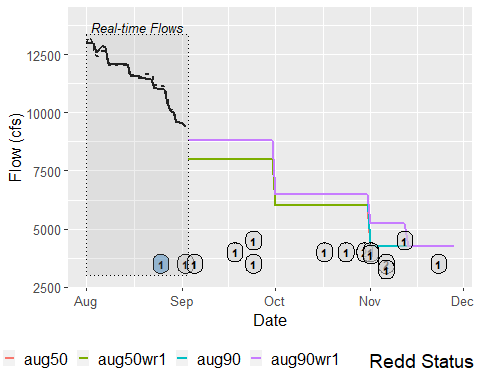
\includegraphics{Real-time-Estimates_Prelim_automated_v4_files/figure-latex/unnamed-chunk-8-1.pdf}
\caption{Actual or estimated emergence dates of SRWC redds and actual or
estimated dewatering flow for the September-October estimated redd
emergence dates as compared to Keswick flow (in cfs) of proposed
management alternatives. Points represent dewatered (De), emerged (Em),
or remaining (Re) redds. Numbers inside of points indicate how many
redds share that estimated emergence date and actual/estimated
dewatering flow. Points that fall above/to the right of a flow
alternative line are expected to be dewatered given that management
alternative is followed. Points that fall below/to the left of/on a flow
alternative line are not expected to be dewatered, given that management
alternative is followed. Shaded gray box shows period of real-time flow
data; dashed black line equals KWK gauge flow and solid black line
equals KES flow (from
\href{https://www.cbr.washington.edu/sacramento/data/query_river_table.html}{SacPas}).}
\end{figure}

\begin{table}

\caption{\label{tab:unnamed-chunk-9}Description of scenarios being considered and compared by the Upper Sacramento Scheduling Team.}
\centering
\begin{tabular}[t]{>{\raggedright\arraybackslash}p{2cm}|>{\raggedright\arraybackslash}p{14cm}}
\hline
Scenario & Descripion\\
\hline
aug50 & Initial rough template scenario put together based on Aug 50\% exceedance forecast. Strategy is to drop to baseflows as quickly as possible while meeting numerous downstream needs, reduce fall-run redd dewatering, conserve water for future years. Does not follow ramping rates\\
\hline
aug90 & Initial rough template scenario put together based on Aug 90\% exceedance forecast.  Strategy is to drop to baseflows as quickly as possible while meeting numerous downstream needs, reduce fall-run redd dewatering, conserve water for future years. Does not follow ramping rates\\
\hline
aug50wr1 & Draft scenario based off of August 50\% forecast. Developed on 8-27-2024 to avoid any winter-run redd dewatering.\\
\hline
aug90wr1 & Draft scenario based off of August 90\% forecast. Developed on 8-27-2024 to avoid any winter-run redd dewatering.\\
\hline
\end{tabular}
\end{table}

\hypertarget{references}{%
\section{References}\label{references}}

Gard, Mark. 2006. Relationships between flow fluctuations and redd
dewatering and juvenile stranding for Chinook Salmon and Steelhead in
the Sacramento River between Kesewick Dam and Battle Creek. 94 pages.

Gosselin, J.L. and W.N. Beer. 2024. Sacramento River Winter-run Chinook
Salmon Redd Dewatering: a Note on Comparing Observed and Predicted.
Central Valley Prediction and Assessment of Salmon (SacPas;
\url{https://www.cbr.washington.edu/sacramento/}). Columbia Basin
Research, School of Aquatic and Fishery Sciences, University of
Washington.

\end{document}
